\chapter{خروجی}
در این قسمت خروجی دستگاه را طی چند اجرای نمونه بررسی ‌می‌کنیم.

\section{تست در روشنایی}

در تصویر زیر می‌توانید مشاهده کنید که چرا سمت چپ خودرو در حضور یک منبع حرارتی جلوی سنسور روشن شده است. همچنین این منبع در سمت چپ خودرو قرار دارد. 

\begin{figure}[H]
	\centering
	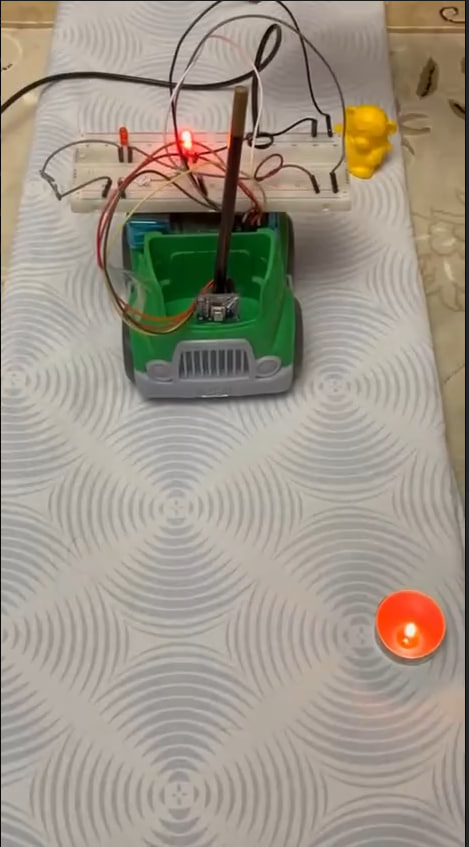
\includegraphics[width=0.5\textwidth]{figs/test_with_lights_on.jpg}
	\caption{تست در روشنایی}
	\label{fig:2}
\end{figure}

در زیر می‌توانید مقداری که اجرای کد، در خروجی استاندار (\lr{stdout}) خود نمایش می‌دهد قبل و بعد از روشن شدن چراغ مشاهده کنید.


آرایه خروجی زیر، قبل از قرار گرفتن شمع در برابر خودرو است. همانطور که می‌بینید تمام دماها‌ی نشان داده شده برای هر پیکسل، تقریبا برابر همان دمای محیط است.
\begin{latin}
\begin{lstlisting}[language=python]
[[23.1 24.4 24.4 23.2 24.7 23.6 23.8 23.8]
 [24.1 24.4 24.9 23.7 24.8 23.5 23.9 23.3]
 [23.6 24.  24.7 24.3 24.7 24.9 24.7 24. ]
 [24.9 23.2 23.7 24.9 24.3 23.6 23.9 23.7]
 [23.3 24.  23.  24.9 24.8 24.2 23.7 23.9]
 [23.8 23.6 23.  23.3 24.9 24.1 24.6 23.6]
 [23.3 23.5 24.8 23.3 23.3 24.2 24.  24.9]
 [23.  23.2 24.7 23.  24.3 23.9 23.  24.6]]
\end{lstlisting}
\end{latin}

اما پس از قرار گیری منبع گرما در برابر خودرو، تغییری ملموس در سمت راست ماتریس خروجی مشاهده می‌شود که نشان از افزایش دما در ناحیه خاصی از محیط دارد. این تغییر دما به احتما قوی می‌تواند مربوط به حضور یک موجود زنده در جلوی خودرو باشد. پس در همین زمان است که دستگاه با روشن کردن چراغ سمت چپ، به راننده هشدار می‌دهد که موجودی زنده در سمت چپ او قرار دارد.
\begin{latin}
\begin{lstlisting}[language=python]
[[23.8 24.8 24.2 24.4 23.4 39.6 40.4 40.2]
 [23.3 23.4 24.4 23.4 23.5 40.4 39.9 39.9]
 [24.6 23.8 23.6 24.2 24.8 39.2 40.4 39. ]
 [23.  24.2 24.9 24.5 23.  47.3 39.2 49.8]
 [23.5 24.  24.1 23.8 24.5 49.9 40.2 48.5]
 [23.4 24.2 24.4 24.4 23.4 39.  40.9 39.3]
 [23.6 23.6 23.7 24.2 23.2 40.6 39.9 39.5]
 [23.5 24.4 23.5 24.8 23.1 40.3 39.7 40.1]]
\end{lstlisting}
\end{latin}


\section{تست در تاریکی}

در تصویر زیر می‌توانید مشاهده کنید که چرا سمت راست خودرو در حضور یک منبع حرارتی جلوی سنسور روشن شده است. همچنین این منبع در سمت راست خودرو قرار دارد. 

\begin{figure}[H]
	\centering
	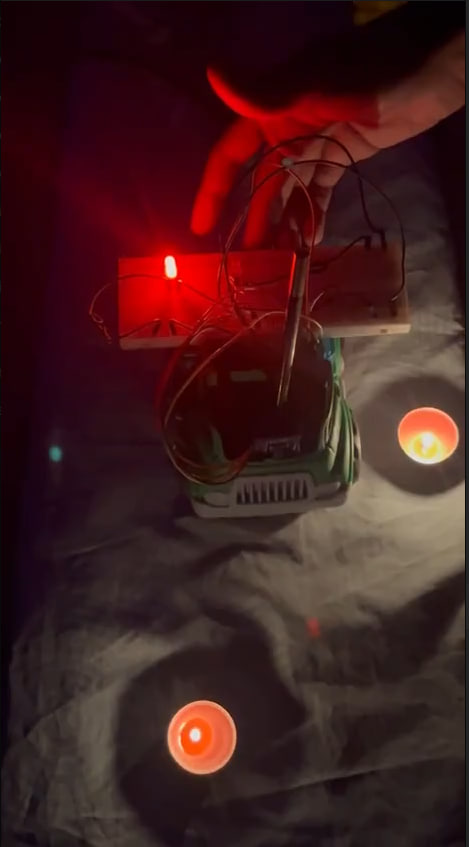
\includegraphics[width=0.5\textwidth]{figs/test_with_lights_off.jpg}
	\caption{تست در تاریکی}
	\label{fig:2}
\end{figure}

در زیر می‌توانید مقداری که اجرای کد، در خروجی استاندار (\lr{stdout}) خود نمایش می‌دهد قبل و بعد از روشن شدن چراغ مشاهده کنید.


آرایه خروجی زیر، قبل از قرار گرفتن شمع در برابر خودرو است. همانطور که می‌بینید تمام دماها‌ی نشان داده شده برای هر پیکسل، تقریبا برابر همان دمای محیط است.
\begin{latin}
\begin{lstlisting}[language=python]
[[23.1 23.  23.7 24.3 24.1 24.7 24.2 23.4]
 [24.2 23.4 24.  24.5 24.7 23.1 23.9 24.9]
 [24.4 23.3 24.9 24.9 24.4 24.9 23.6 23.1]
 [24.4 23.7 23.4 24.7 23.9 24.3 23.6 23.3]
 [24.4 24.3 23.3 23.1 24.2 23.9 23.5 23.4]
 [23.5 23.2 24.8 23.8 23.5 23.7 23.7 24.1]
 [23.6 23.7 23.5 24.5 23.1 23.8 24.6 23. ]
 [24.1 24.2 24.2 24.4 23.2 24.1 24.4 24. ]]
\end{lstlisting}
\end{latin}

اما پس از قرار گیری منبع گرما در برابر خودرو، تغییری ملموس در سمت چپ ماتریس خروجی مشاهده می‌شود که نشان از افزایش دما در ناحیه خاصی از محیط دارد. این تغییر دما به احتما قوی می‌تواند مربوط به حضور یک موجود زنده در جلوی خودرو باشد. پس در همین زمان است که دستگاه با روشن کردن چراغ سمت راست، به راننده هشدار می‌دهد که موجودی زنده در سمت راست او قرار دارد.
\begin{latin}
\begin{lstlisting}[language=python]
[[45.1 45.  45.7 46.3 24.1 24.7 24.2 23.4]
 [46.2 45.4 46.  46.5 24.7 23.1 23.9 24.9]
 [46.4 45.3 46.9 46.9 24.4 24.9 23.6 23.1]
 [51.4 50.7 45.4 46.7 23.9 24.3 23.6 23.3]
 [54.4 53.3 45.3 45.1 24.2 23.9 23.5 23.4]
 [45.5 45.2 46.8 45.8 23.5 23.7 23.7 24.1]
 [45.6 45.7 45.5 46.5 23.1 23.8 24.6 23. ]
 [46.1 46.2 46.2 46.4 23.2 24.1 24.4 24. ]]
\end{lstlisting}
\end{latin}



\chapter{جمع‌بندی}
در این پروژه به پیاده‌سازی سیستم دید در شب اتومبیل پرداختیم که به راننده برای جلوگیری از سانحه در محیط‌های تاریک کمک می‌کند. در این سیستم با استفاده از سنسور دوربین حرارتی که از طریق جذب مادون قرمز عمل می‌کند و همچنین واحد پردازشی رزپری‌پای، حضور یک موجود زنده جلوی دید راننده را تشخیص و به کمک چرا‌غ‌ها به اون هشدار دادیم. 

در کنار طراحی کلی و نحوه پیاده‌سازی، تمام کد‌های مربوط به این محصول نیز به صورت متن باز در گیتهاب پروژه قراره گرفته است و هرکسی می‌تواند با کمک این کدها به بهبود و ارتقاء این سیستم کمک کند و یا با الهام از آن، پیاده سازی خاص خودش را ارائه دهد. 

آنچه محصول ما را از دیگر محصول‌ها متمایز می‌کند قیمت بسیار پایین تمام‌شده‌ی ‌آن است که می‌توان حتی بیشتر آن را کاهش داد. به عنوان مثال با استفاده از آردوینو به جای رزپری و همچنین استفاده از چراغ‌های خودرو به جای چراغ‌های مجزا برای سیستم. حتی می‌توان در هنگام پیاده‌سازی این سیستم برای خودرو، کد آن را به عنوان یک نرم افزار در اختیار کامپیوتر خودرو قرار داد و تمام مسئولیت‌های رزپری را به کامپیوتر اتومبیل سپرد.